\chapter{Implementación}\label{cap:implementacion}

Como se ha descrito en el capítulo anterior, la propuesta de arquitectura consiste en una arquitectura heterogénea con las funcionalidades de cómputo intensivo implementadas en C++ y las funcionalidades de alto nivel implementadas mantenidas del prototipo. Debido a la diferencia en tecnologías entre las partes de la arquitectura, resulta necesaria la implementación de un cauce de comunicación entre las partes. El entorno de NodeJS nos presenta varias posibilidades para hacer esto como se explicará más adelante. De esta manera, la base de código se dividirá en tres paquetes:

\begin{enumerate} 
    \item \textbf{genomus-core}\cite{genomus-core}: Una biblioteca de C++ que implementa el modelo de datos y de cómputo de GenoMus
    \item \textbf{genomus-core-js}\cite{genomus-core-js}: Un paquete de NPM conformado por un módulo nativo de NodeJS que expone la API de interación entre el runtime de javascript y la biblioteca de C++.
    \item \textbf{genomus-js}: Un paquete de NPM que mantiene las funcionalidades de entrada/salida del prototipo.
\end{enumerate}

Un diagrama de esta arquitectura se puede ver en la figura \ref{fig:arquitectura}.

Debido a que es secundario al propósito de este proyecto, se ha decidido dejar el paquete \textbf{genomus-js} para trabajos futuros, por lo que esta implementación solo contará con las dos primeras librerías.

\begin{figure}
    \centering
    \fbox{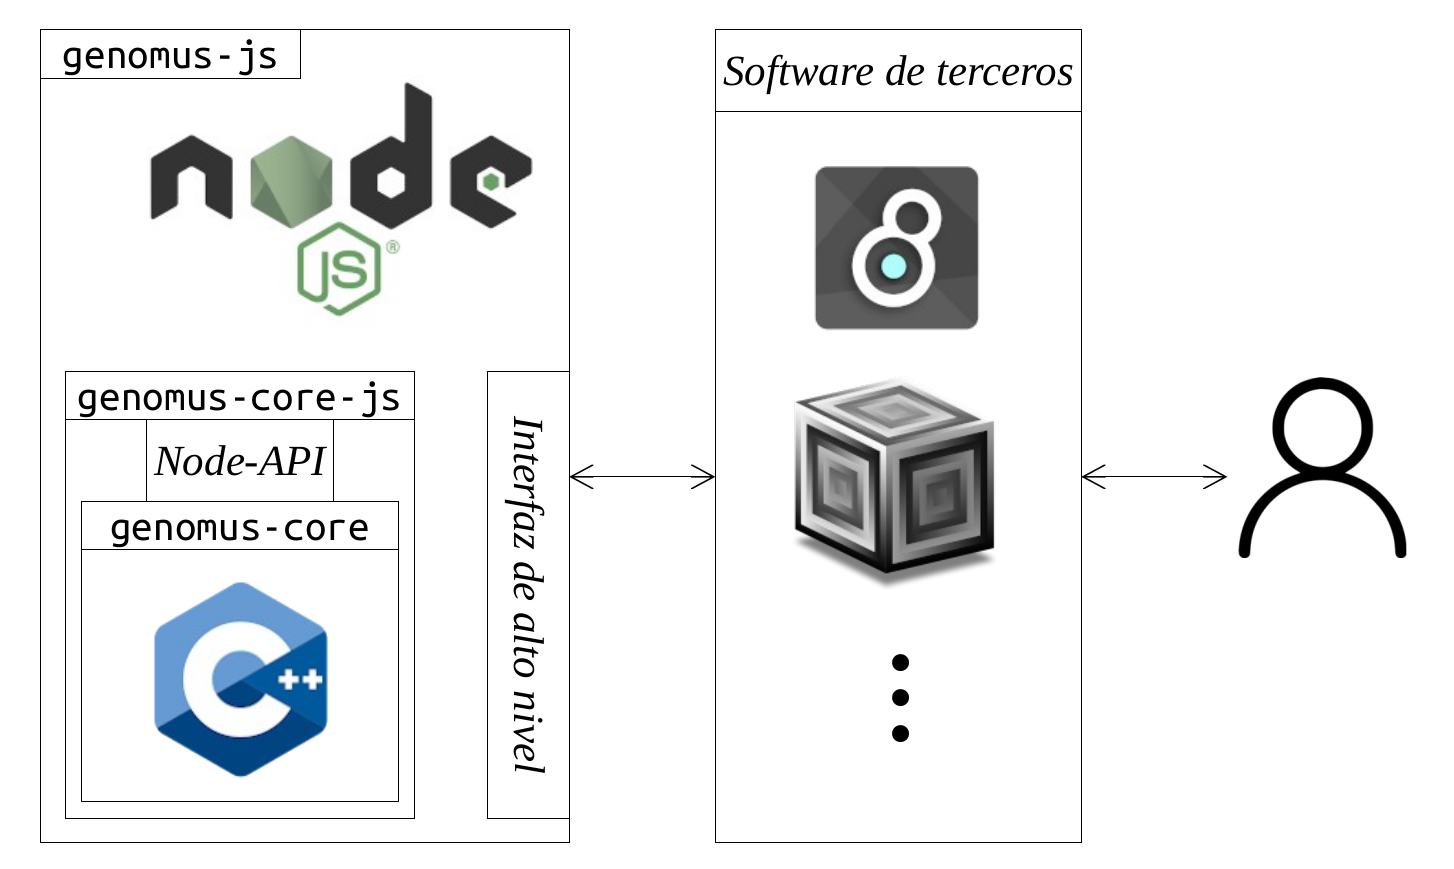
\includegraphics[width=\textwidth]{imagenes/diagrama-arquitectura.png}}
    \caption{Diagrama de arquitectura del software.}
    \label{fig:arquitectura}
\end{figure}

\section{Entorno de desarrollo}

Para el desarrollo se ha escogido VSCode, debido a su soporte de las diferentes tecnologías que se han utilizado en este proyecto y a la capacidad de desplegar un entorno de desarrollo funcional en cualquier máquina mediante la inclusión de archivos de configuración en los repositorios. Las tecnologías a utilizar en los entornos de desarrollo facilitadas por VSCode son las siguientes:

\begin{itemize}
    \item \verb|ClangD| como servidor de lenguaje para \verb|C++|. Está basado en el compilador de \verb|C++| de Clang\footnote{Más información en \url{https://clang.llvm.org/}}, siendo parte del proyecto LLVM\footnote{Más información en \url{https://llvm.org/}}. Proporcionado a través del paquete homónimo de VSCode\footnote{Documentación en \url{https://marketplace.visualstudio.com/items?itemName=llvm-vs-code-extensions.vscode-clangd}}
    
    \item \verb|CMake| como \textit{toolkit} de compilación de C++. Proporcionado por VSCode a través del paquete \verb|CMake Tools|\footnote{Documentación en \url{https://marketplace.visualstudio.com/items?itemName=ms-vscode.cmake-tools}}
    
    \item Automatización de lanzamiento de tests y depurado. VSCode nos proporciona con funcionalidades de automatización a través de la configuración de su archivo de configuración \verb|launch.json|\footnote{Documentación en \url{https://code.visualstudio.com/docs/cpp/launch-json-reference}}
    
    \item Servidores de lenguaje para \verb|javascript| y \verb|typescript| incorporados por defecto en VSCode
\end{itemize}

La configuración del entorno de desarrollo se puede consultar en los archivos de configuración pertinentes en los repositorios (\url{https://github.com/mipdr/genomus-core} y \url{https://github.com/mipdr/genomus-core-js}).

\section{genomus-core}

\verb|genomus-core| implementa el modelo de datos y de cómputo de GenoMus. Como se ha enunciado previamente, la base de código está liberada bajo licencia MIT y se puede consultar en un repositorio público alojado en Github\cite{genomus-core}.

\subsection{Dificultades de implementación en C++}\label{ssec:dificultades}

El modelo de cómputo de GenoMus está intrínsecamente basado en el paradigma de programación funcional. Esto hace que una implementación en \verb|C++| no sea trivial por la necesidad de los siguientes constructos:

\begin{itemize}
    \item \textbf{Declaración de funciones en tiempo de ejecución.} Las funciones de cómputo disponibles deben ser declarables en tiempo de ejecución. Ya que las funciones disponibles al modelo de cómputo son dependientes del estado del programa, es ideal que estas se puedan declarar dinámicamente en tiempo de ejecución. En la actual implementación, se proporciona una serie de funciones instanciadas en tiempo de carga.
    
    \item \textbf{Polimorfismo funcional.} Necesitamos construcciones que doten al modelo de cómputo de polimorfismo declarado en tiempo de ejecución. Debe ser posible no solo declarar nuevas funciones en tiempo de ejecución, sino también declarar nuevos tipos a usar como parámetros o salidas. Esto elimina de la ecuación casi todos los constructos que \verb|C++| ofrece para conseguir polimorfismo dinámico, ya que el dominio del polimorfismo debe ser conocido en tiempo de compilación en \verb|C++|.
    
    \item \textbf{Árboles funcionales declarables y evaluables.} Toda instancia de cómputo debe no solo ser computable sino también almacenable. La instancia de árbol funcional debe existir independientemente de su evaluación. Así, una función de cómputo será un objeto invocable o functor cuya invocación contribuirá a la declaración del árbol funcional en memoria. Esto, además de ser necesario para el funcionamiento del software, posibilita el diseño de algoritmos de cómputo sobre el árbol funcional más allá del típico recorrido por profundidad\footnote{
        Refiriéndose a los métodos de optimización propios de lenguajes comparativos, como la máquina de reducción de grafos de GHC\cite{haskell-wiki-STG}.
    }.
    
    \item \textbf{Funciones enumerables en tiempo de ejecución.} Las funciones de cómputo disponibles en tiempo de ejecución deben ser enumerables en tiempo de ejecución. Esto significa que deben ser almacenables en un contenedor en tiempo de carga.
\end{itemize}

Todas estas características son bien incompatibles con la metodología de desarrollo orientado a objetos estándar de \verb|C++| o bien incompatibles con la máxima del proyecto de ser asequible para programadores amateur, si pretendemos seguir las buenas prácticas de \verb|C++|. Por este motivo se toma la decisión de alejarse de la práctica principal de polimorfismo definida en los últimos estándares de \verb|C++|\footnote{
    Refiriéndose a constructos definidos en los estándares de C++11 a C++17 como \textit{variadic templates}, \textit{reference semantics} o \textit{parameter packing}. 
} para realizar una implementación mixta entre orientada a objetos clásica y orientada a prototipos. 

Lo que nos aporta conceptualmente el diseño orientado a prototipos es la posibilidad de manejar parcialmente el tipado de nuestros objetos en tiempo de ejecución. Por otra parte, la principal desventaja que nos trae es la existencia de errores de tipado no conocidos por el compilador, lo cual es natural cuando lo que buscamos es precisamente declarar funciones de tipado arbitrario en tiempo de ejecución.

De esta manera se nos presenta un compromiso entre la seguridad del código y la legibilidad de este. La implementación propuesta busca maximizar la legibilidad y flexibilidad del código minimizando la cantidad de comprobaciones de tipado en tiempo de ejecución. Además, se plantea mitigar el riesgo del tipado dinámico mediante la creación de tests de integración.

\subsection{Modelo de datos}

Como se ha explicado en el capítulo \ref{cap:descripcion}, el modelo de datos de GenoMus define dos tipos de representación de datos musicales a distintos niveles de abstracción, a los cuales los llama \textbf{genotipos} y \textbf{fenotipos}.

Un genotipo y un fenotipo musicales son conceptualmente muy diferentes. El genotipo define una serie de transformaciones sobre materiales musicales básicos, mientras que el fenotipo define instancias de música. A pesar de esta diferencia conceptual, ambos conceptos son representables como grafos dirigidos. Se explicará a continuación la propuesta de implementación de estas estructuras.

\subsubsection{Instancias de música: la partitura}

Para hablar de la estructura conceptual de los fenotipo debemos hablar necesariamente de la estructura de representación usual de datos musicales, es decir la partitura. Con el término \textit{partitura} nos referimos no a la tradicional hoja de papel con notación musical, sino a la estructura de esta. Estructura que vemos presente a lo largo de las diferentes representaciones analógicas o digitales de datos musicales. Una paritura \textit{score} consiste en una serie de grupos simultáneos de eventos consecutivos. Podemos deinir esta estructura a nivel conceptual de la siguiente manera:

\begin{itemize}
    \item \textit{Evento}: equivale a la nota musical en la mayoría de los casos. Es el grano mínimo de información musical. Un evento ocurre en un intervalo de tiempo acotado y está definido por una seria de parámetros como pueden ser la altura, intensidad o duración (en el caso de estar hablando de eventos sonoros).
    
    \item \textit{Voz}: Conjunto de Eventos consecutivos en el tiempo.
    
    \item \textit{Partitura}: Conjunto de Voces que ocurren simultáneamente.
\end{itemize}

Esta estructura corresponde a la \textit{Partitura} tradicional sobre papel, y a la que utiliza GenoMus.

\subsubsection{Fenotipos como árboles de profundidad acotada}

La definición conceptual de Fenotipo es la de \textit{instancia de música}. Es decir datos que pueden ser traducidos a un formato legible por un humano o instrumento virtual sin necesidad de ninguna evaluación de los datos. Esto supone que la estructura del fenotipo es dependiente de la estructura de los datos aceptados por un software de salida. En la representación tradicional de la música, un \textit{evento} equivale a una \textit{nota}, la cual está definida por parámetros escalares. La representación de un evento en un instrumento virtual particular podría no solo estar definida por un conjunto diferente de parámetros, sino incluso contener parámetros no escalares. Debido a esto se propone la implementación del fenotipo como un árbol de profundidad acotada conforme a lo establecido por la jerarquía de tipos fenotípicos definida.

\subsubsection{Implementación de fenotipos en C++}

La implementación en \verb|C++| de esta estructura es la primera instancia de diseño orientado a prototipos del proyecto. Se define el TDA \verb|EncodedPhenotype| descrito en la figura \ref{fig:decoded_phenotype_hpp}, cuyas instancias almacenarán su propio tipo y comprobarán que sus hijos son del tipo correcto. De esta manera, la estructura de datos \verb|EncodedPhenotype| es de tipado homogéneo en tiempo de compilación, ya que todos sus nodos corresponden a instancias del prototipo. A partir de este TDA, se definen diferentes prototipos que fijan los valores de tipo y de tipo hijo. Esto convierte el esfuerzo de definir estructuras de fenotipo alternativas en una mera definición de prototipos que definan los tipos que estructuran el fenotipo.
\\ \\
Pero, ¿por qué se ha implementado el polimorfismo de tiempo de ejecución a través de prototipos y no a través de la herencia de clases que nos proporciona \verb|C++|? La respuesta recae sobre una de las máximas del proyecto: la mantenibilidad del código por un programador amateur. El sistema de herencia y polimorfismo de \verb|C++| es muy potente, pero excesivamente complejo incluso para programadores con experiencia en el paradigma orientado a objetos. Los conceptos de sobrecarga de métodos y las \textit{reference semantics}\footnote{Las \textit{Reference semantics} o semánticas de referencia son una serie de constructos del lenguaje C++ para manejar instancias de objetos a través de punteros a estos, constructos como \textit{unique\_ptr} o \textit{make\_shared}. Esto es especialmente útil para definir contenedores polimórficos, ya que una instancia de una clase hija no puede almacenarse en memoria como una instancia de la clase padre, pero un puntero a una instancia de la clase hija sí que puede pasar por un puntero de tipo padre. Artículo que las explica en detalle: \url{https://learnmoderncpp.com/2021/02/26/reference-semantics-for-c-classes/}. Las \textit{reference semantics} son complejas y requieren de estudio para entenderlas y manejarlas, por lo que las evitaremos en este proyecto.} difieren de los conceptos polimórficos de implementan otros lenguajes del paradigma como \verb|java|, \verb|python| o el propio \verb|javascript|. Pero no es todo un intento de evitar constructos complejos. El establecimiento de la estructura fenotípica como prototipo permite que la declaración de nuevas estructuras fenotípicas no incluya alteraciones al sistema de tipado del código. Permite declarar dinámicamente en tiempo de ejecución nuevas estructuras fenotípicas.

\begin{figure}
    \centering
    \begin{lstlisting}[language=cpp]
class EncodedPhenotype {
    ...
    
    private:
        EncodedPhenotypeType _type;
        EncodedPhenotypeType _child_type;
        std::vector<EncodedPhenotype> _children;
        
    ...
};

EncodedPhenotype Event(std::vector<EncodedPhenotype> parameters);
EncodedPhenotype Voice(std::vector<EncodedPhenotype> parameters);
EncodedPhenotype Score(std::vector<EncodedPhenotype> parameters);
    \end{lstlisting}
    \caption{Declaración del TDA EncodedPhenotype y de los prototipos que lo implementan.}
    \label{fig:decoded_phenotype_hpp}
\end{figure}


\subsubsection{Funciones de transformación musical}

Las funciones de GenoMus son el soporte del modelo de cómputo; en otras palabras, son los operadores que dan riqueza al abanico de posibilidades creativas que el software ofrece al usuario. La implementación del sistema de cómputo asociado a estas funciones se explicará en el punto \ref{ssec:modelo_computo}. En esta sección se hablará de la necesidad de establecer una estructura de datos para representar \textit{expresiones}, es decir constructos sintácticos que codifican una instancia de cómputo que ocurre al evaluarlos. 

Las expresiones de GenoMus cuentan con dos tipos de elementos: funciones y datos hoja numéricos. Las expresiones se construyen en la manera usual: notación prefija con paréntesis englobando los parámetros de los operadores. Por este motivo la representación en memoria más intuitiva es la equivalente a un árbol de sintaxis abstracto\cite{dragon-book-ast}.

\subsubsection{Genotipos como grafos dirigidos acíclicos}

No obstante, GenoMus contiene una funcionalidad que hace del grafo acíclico dirigido la mejor estructura de datos para representar genotipos. Esta funcionalidad son las autoreferencias. Una autoreferencia es una referencia a otro nodo del árbol de sintaxis, y será evaluada de manera equivalente al nodo que referencia. (véase la figura \ref{fig:autoreferencia}).

\begin{figure}
    \centering
    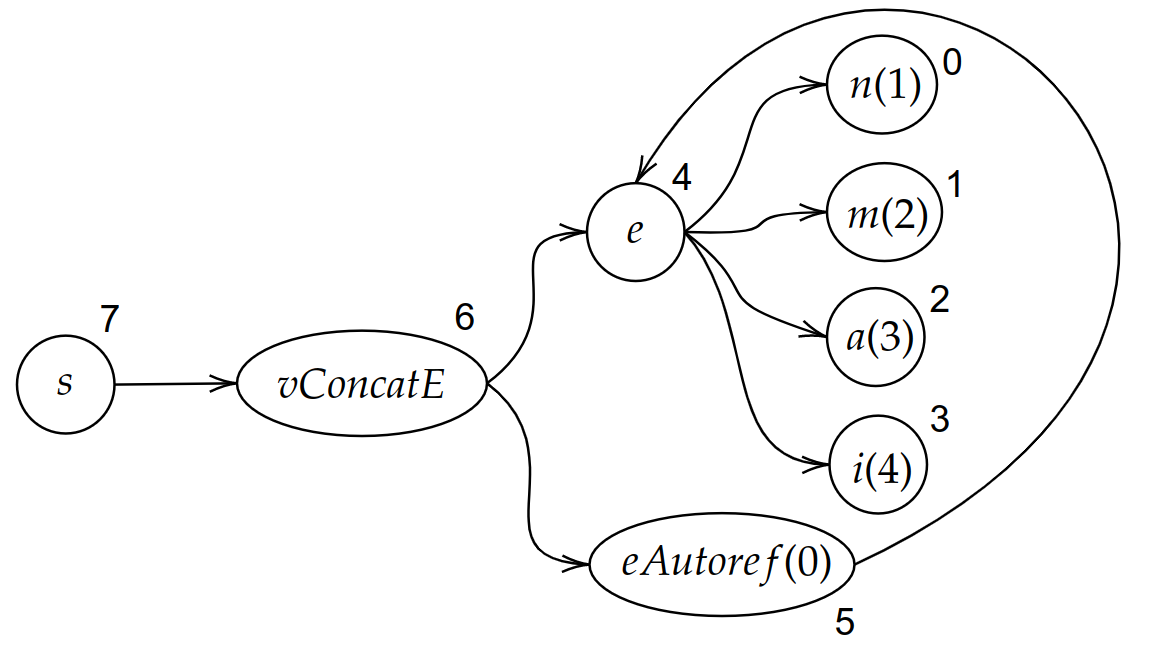
\includegraphics[width=\textwidth]{imagenes/autoreference.png}
    \caption{Diagrama de autoreferencia.} En este diagrama podemos ver la estructura de un genotipo con una autoreferencia de tipo \textit{evento}: eAutoref. Para asegurar que el grafo es acíclico, una autoreferencia es válida únicamente cuando referencia a un nodo con índice menor en un recorrido profundidad-primero del árbol, indicados a la derecha de los nodos. Los detalles de implementación se pueden consultar en el código del proyecto.
    \label{fig:autoreferencia}
\end{figure}

Se plantea la implementación de un grafo dirigido acíclico con funciones como nodos y referencias basadas en índices de un contenedor indexado de nodos. 

 
\subsubsection{Implementación de Genotipos en C++}

De esta manera, los genotipos son implementados como un grafo que tiene funciones por nodos y la relación ``ser parámetro de'' como aristas. Se propone la implementación de dos tipos de datos para esto. El primero es el TDA \verb|GFunction|, el cual representa una función de GenoMus. El segundo es el TDA \verb|GTree|, el cual representa el grafo sintáctico. La implementación de \verb|GFunction| será descrita en detalle en el siguiente punto, por ahora solo necesitamos saber que es un objeto invocable que representa una función de GenoMus. Se puede consultar una declaración simplificada de esta estructura de tipos en la figura \ref{fig:dec_gen_hpp}. 

Las instancias de árboles sintácticos de funciones de GenoMus se instancian en memoria de la siguiente manera:

\begin{itemize}
    \item Los nodos del árbol se almacenan en el contenedor \verb|GTree::tree_nodes|.
    \item Los arcos del árbol se almacenan en las instancias de GTree. Cada nodo declara un array de referencias a sus hijos.
    \item Los literales numéricos son almacenados por las instancias de GTree. Si un nodo tiene como hijo un literal numérico, este será almacenado en el campo \verb|GTree::_leaf_value|.
\end{itemize}

\begin{figure}
    \centering
    \begin{lstlisting}[language=cpp]
class GTree {
    public:

    class GTreeIndex {
        private:
            size_t _index;
            
        ...
    };

    class GFunction {
        ...
        
        private:
            std::string _name;
            size_t _index;
            std::vector<EncodedPhenotypeType> _param_types;
            EncodedPhenotypeType _output_type;
            std::function<enc_phen_t(std::vector<enc_phen_t>)> _compute;
            
        ...
    };
    
    private:
        GFunction& _function;
        std::vector<GTreeIndex> _children;
        double _leaf_value;
        
        ...
    public:
        static std::vector<GTree> tree_nodes;
        
        ...

        enc_phen_t evaluate();
        std::vector<double> toNormalizedVector();
};
    \end{lstlisting}
    \caption{Declaración de los TDA de genotipos.} \textit{GFunction} es el TDA que representa funciones de GenoMus. \textit{GTree} es el TDA que representa un nodo de un árbol sintáctico de funciones de GenoMus. \textit{GTreeIndex} es un TDA auxiliar para facilitar el acceso por referencia a instancias de \textit{GTree}.
    \label{fig:dec_gen_hpp}
\end{figure}

\subsection{Modelo de cómputo}\label{ssec:modelo_computo}

Como se ha explicado en el capítulo 3, el modelo de cómputo de GenoMus consiste en los algoritmos de evaluación de expresiones genotípicas en fenotipos. El algoritmo de evaluación es equivalente al de cualquier evaluador de árbol sintáctico funcional, siendo la evaluación de un árbol una función pura. Existen una serie de excepciones en forma de la existencia de funciones no puras, lo cual acarrea problemas para asegurar la pureza de la evaluación del árbol. Estas funciones no puras son las siguientes:

\begin{itemize}
    \item \textbf{Funciones aleatorias}. Por definición producen resultados diferentes en cada evaluación. Si una función aleatoria está contenida en un \verb|GTree|, su evaluación en el contexto de la evaluación del árbol completo debe dar siempre el mismo resultado. Esto se consigue mediante el guardado del resultado de la primera evaluación de la función en el estado del árbol.
    
    \item \textbf{Autoreferencias}. Por definición su evaluación es dependiente de su inclusión en un árbol sintáctico. Una autoreferencia no existe como función evaluable por sí misma. Al depender del estado del árbol, no afecta a la pureza de la evaluación del árbol completo.
\end{itemize}

\subsection{Utilidades: Parser y CLI}

Como se ha mencionado previamente, el desarrollo de la biblioteca \verb|genomus-core| ha hecho uso de tests de integración para emular la interacción con otro software en casos de uso reales. No obstante estos tests no son adecuados para emular interacciones sobre la marcha durante el proceso de desarrollo. Es por esto que se implementa un parser de expresiones GenoMus y un intérprete de línea de comandos que hace uso de este. Con estas utilidades, la biblioteca es fácilmente utilizable desde la propia consola. 

GenoMus se ha definido como un metalenguaje por las condiciones de implementación del prototipo. El uso fundamental del uso de la principal funcionalidad de metaprogramación de javascript, la función \verb|eval| (descrito en la sección \ref{ssec:eval_evil}), pone el diseño del código del prototipo como uno de metaprogramación. Como se ha mencionado previamente, la implementación propuesta de \verb|genomus-core| requiere de la desaparición de la metaprogramación. \verb|C++| no es un lenguaje con funcionalidades nativas de metaprogramación, ya que el parseo y compilación de expresiones que esto implica se alejan de la filosofía del lenguaje.

\subsubsection{El parser}

Se propone la implementación de un parser de expresiones representativas de genotipos de GenoMus. La entrada de este parser es una cadena de texto y la salida es la estructura de datos que representa el genotipo en memoria. Afortunadamente, la comprobación dinámica de tipado en estas estructuras que se ha mencionado previamente asume la mayor parte de la responsabilidad de la comprobación de la validez de una entrada de texto. El parser deberá realizar un análisis de validez sintáctica, ya que el análisis semántico recae sobre la construcción de la estructura en memoria. 

El funcionamiento del parser sigue la lógica básica de cualquier parser perteneciente al frontend de un compilador. En primer lugar, recorre la entrada de texto para extraer un array de tokens, a partir del cual construye un AST o árbol abstracto de sintaxis (Abstract Syntax Tree). Citando la sección \textit{2.5.1 Abstract and Concrete Syntax} del mítico "Dragon Book"\cite{dragon-book-ast}:

\begin{quote}
    \textit{
    A useful starting point for designing a translator is a data structure called an abstract syntax tree. In an abstract syntax tree for an expression, each interior node represents an operator; the children of the node represent the operands of the operator. More generally, any programming construct can be handled by making up an operator for the construct and treating as operands the semantically meaningful components of that construct
    }
\end{quote}

El parser realiza una separación de la cadena de texto en tokens, los cuales recorre formando el AST. En esta etapa se realizan comprobaciones sintácticas, que se reducen principalmente a comprobar la correcta disposición de paréntesis en la entrada. Esto se puede ver en la sesión interactiva ilustrada en la figura \ref{fig:interpreter}

Tras la construcción del AST, el parser realiza un recorrido de este para interpretar su semántica y construir una instancia de \verb|GTree| que lo represente. En esta etapa se realiza una traducción de tokens a funciones de GenoMus o literales, y se emiten errores en el caso de que se hayan introducido tokens inválidos. Esto se puede ver en la sesión interactiva ilustrada en la figura \ref{fig:interpreter} 

Se puede ver un esquema ilustrativo del funcionamiento del parser en la figura \ref{fig:parser}. 


\begin{figure}
    \centering
    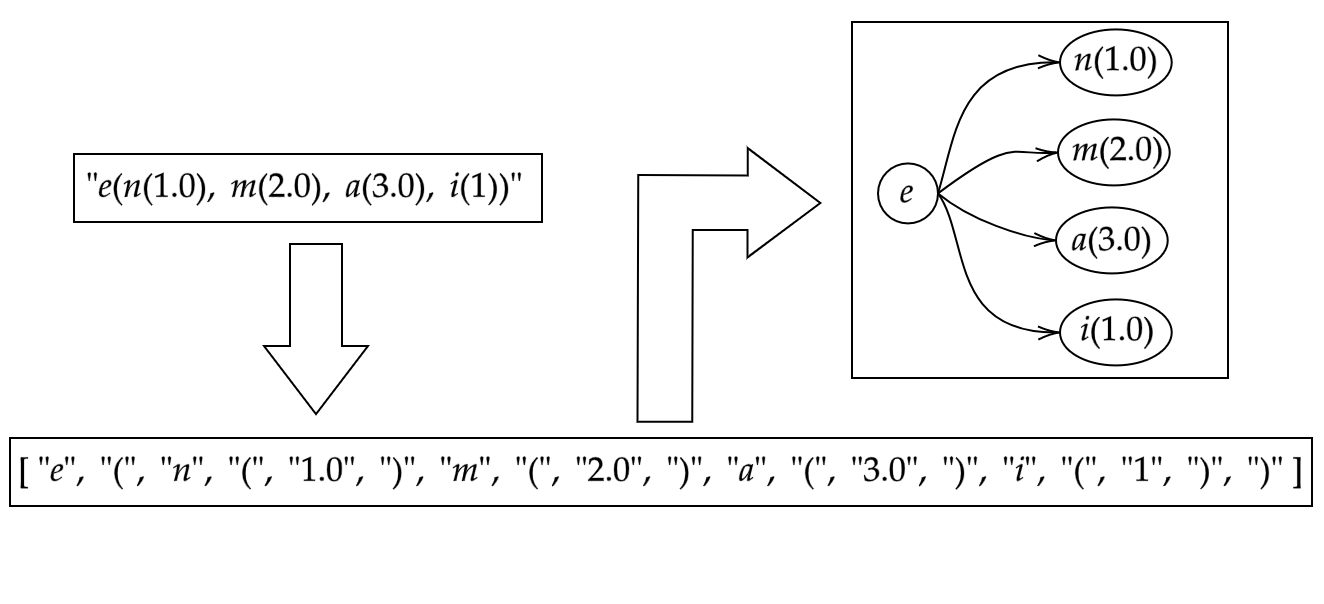
\includegraphics[width=\textwidth]{imagenes/parser.png}

    \caption{Procedimiento de parseo simplificado.} En este esquema podemos ver las dos transformaciones principales que realiza el parser. En primer lugar, la identificación de tokens en la entrada. En segundo lugar la construcción de una instancia de GTree.
    \label{fig:parser}
\end{figure}

\subsubsection{El intérprete}

Una vez implementado el parser de expresiones, se propone la implementación de un intérprete de línea de comandos, dado que la mayor parte del trabajo estaba ya hecho con el parser. Se implementa una interfaz de línea de comandos capaz de evaluar:

\begin{itemize}
    \item Expresiones GenoMus. 
    \item Comandos definidos por el intérprete. En la actual implementación se definen los siguientes comandos:
    \begin{itemize}
        \item \verb|\list| para listar las funciones disponibles.
        \item \verb|\list_verbose| para listar las funciones disponibles con datos asociados como su tipo o el tipo de sus parámetros.
        \item \verb|\q| para terminar la sesión interactiva.
    \end{itemize}
\end{itemize}

El intérprete cuenta con un mensaje de bienvenida y con un prompt que indica la espera de entrada de texto. En la figura \ref{fig:interpreter} se puede ver un ejemplo de sesión interactiva con el intérprete.
 
\begin{figure}
    \centering
    \fbox{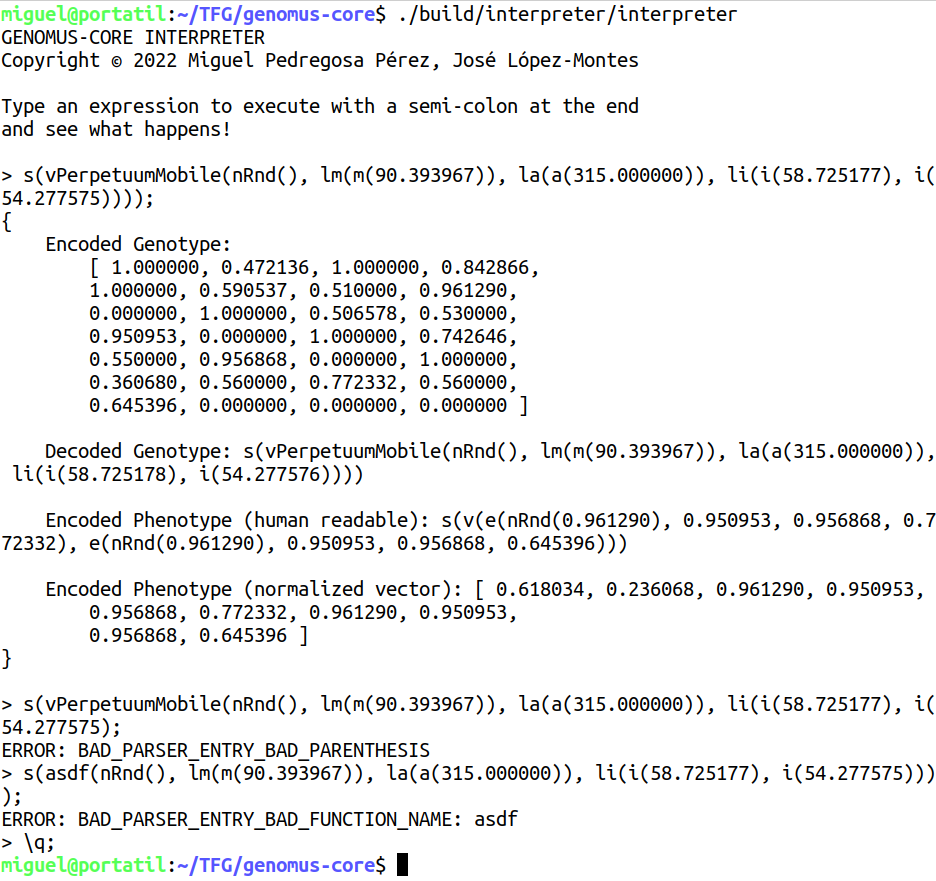
\includegraphics[width=\textwidth]{imagenes/interpreter.png}}
    \caption{Ejemplo de una sesión del intérprete.} En esta figura se ilustra una sesión interactiva con el intérprete con entradas de teclado correspondientes a variaciones de la expresión generada aleatoriamente \textit{s(vPerpetuumMobile(nRnd(), lm(m(90.393967)), la(a(315.000000)), li(i(58.725177), i(54.277575))))}. Podemos ver cómo la eliminación de algunos paréntesis finales en la segunda entrada de teclado produce un error sintáctico durante la construcción del AST. También podemos ver como una alteración del nombre de una función en la terera entrada de teclado nos da un error de semántica, ya que \textit{asdf} no es un token conocido por el intérprete. También se puede ver la utilización del comando de terminación de la sesión.
    \label{fig:interpreter}
\end{figure}
 
\subsection{Tests automatizados: GTest}

El proceso de desarrollo de \verb|genomus-core| ha sido acompañado de un proceso de TDD, como ya se ha indicado previamente. Se ha implementado un framework de tests de integración automatizado desde cero llamado GTest, el cual maneja los siguientes conceptos:

\begin{itemize}
    \item \textbf{Test case}. Conforma el grano mínimo de funcionalidad a testear. Puede decirse que es un test unitario.
    
    \item \textbf{Test}. Conformado por un conjunto de \textit{test cases}, se encarga de testear un grupo funcional del software. Puede decirse que es un test de integración.
\end{itemize}

En el extracto de código de la figura \ref{fig:gtest} podemos ver un ejemplo de la declaración de un test con varios \textit{test cases}. El programador declara test cases a los que opcionalmente les puede proporcionar un cauce de salida, en el cual el test case escribe información útil para el programador en caso de que el test falle. Además, el programador puede declarar acciones a ejecutar al comienzo del test, tras finalizar el test y al comienzo de cada test case.

GTest proporciona una salida de texto en la que informa al programador del éxito o fracaso de los tests declarados, mostrando también el tiempo de ejecución de los diferentes tests, como se puede ver en la figura \ref{fig:tests_output}.

\begin{figure}
    \centering
    \begin{lstlisting}[language=cpp]
#include <iostream>
#include <stdexcept>

#include "genomus-core.hpp"
#include "testing_utils.hpp"

GTest ParserTest = GTest("Parser test")

    .before([]() { init_genomus(); })
    .beforeEach([]() { GTree::clean(); })
    .after([]() { GTree::clean(); })

    .testCase("Check parser tokens", [](ostream& os) {
        std::string entry = "vConcatV(vConcatE(e(n(1.0), m(2.0), a(3.0), i(1)), eAutoref(0)), vConcatE(eAutoref(1), eAutoref(2)))";
        dec_gen_t tree = parseString(entry);

        os << "Entry: " << entry << "\n\n";
        os << "Decoded Genotype: " << tree.toString() << "\n\n";
        os << "Encoded Phenotype: " << tree.evaluate().toString() << "\n\n";
    })

    .testCase( ... 
        ...
    );
\end{lstlisting}
    \caption{Declaración de un test mediante GTest.}
    \label{fig:gtest}
\end{figure}

\begin{figure}
    \centering
    \fbox{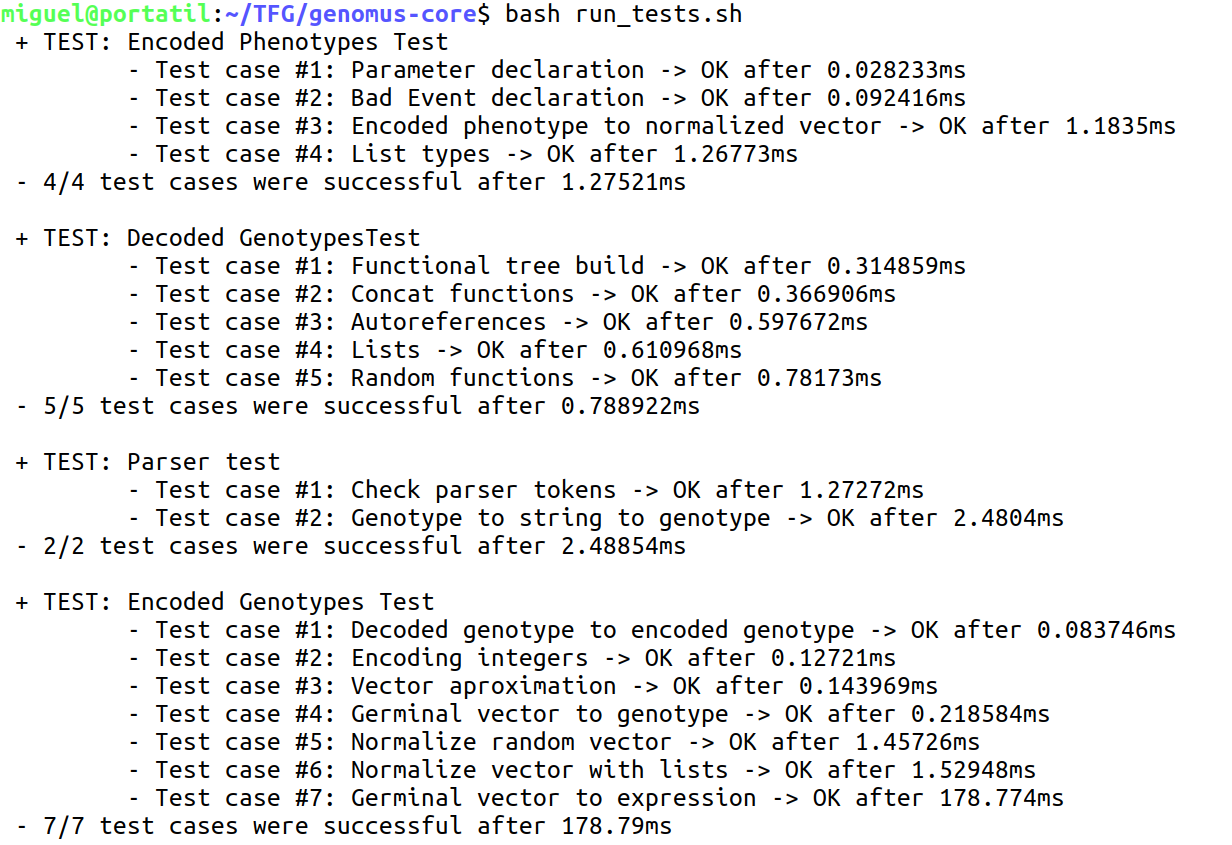
\includegraphics[width=\textwidth]{imagenes/tests_output.png}}
    \caption{Resultado del lanzamiento de los tests automáticos del proyecto.}
    \label{fig:tests_output}
\end{figure}


%%%%%%% GENOMUS-CORE-JS %%%%%%%%

\section{genomus-core-js}

\verb|genomus-core-js| se presenta como el paquete de JS que expone la interfaz de comunicación con el modelo de cómputo de \verb|genomus-core|. Para esto se hace uso de las siguientes tecnologías:

\begin{itemize}
    \item \textbf{Node-API}: como librería para crear objetos de \verb|javascript| desde C++. 
    \item \textbf{Node-GYP}: toolkit para la construcción de proyectos que utilizen Node-API. Basado en el sistema de construcción GYP\footnote{
        GYP es un meta-sistema de construcción utilizado para generar sistemas de construcción de software. Más información en su página oficial (\url{https://gyp.gsrc.io/}).
    }.
\end{itemize}

La elección de \verb|Node-API| como interfaz de abstracción nativa de NodeJS entre otras posibilidades como \verb|V8|\cite{V8-API} o \verb|nan|\cite{node-nan} recae sobre la estabilidad de la primera a través de las diferentes versiones de NodeJS. Como bien explica la documentación oficial de NodeJS\cite{node-addon-docs}:

\begin{quote} \textit{
    Node-API is an API for building native addons. It is independent from the underlying JavaScript runtime (e.g. V8) and is maintained as part of Node.js itself. This API will be Application Binary Interface (ABI) stable across versions of Node.js. It is intended to insulate addons from changes in the underlying JavaScript engine and allow modules compiled for one version to run on later versions of Node.js without recompilation.
}\end{quote}

La estabilidad de la interfaz binaria hace \verb|Node-API| ideal para nuestro propósito.
 
\subsection{Desarrollo de un paquete NPM con tipado de Typescript}

Se ha decidido desarrollar \verb|genomus-core-js| como un paquete de Typescript nativo, es decir programado en Typescript. Las principales ventajas de esto son las dadas por un sistema de tipado estático cualquiera, es decir la facilitación del mantenimiento del código y la seguridad añadida de realizar comprobaciones de tipado en tiempo de compilación. Las desventajas asociadas son el aumento del tiempo de instalación del paquete, ya que la compilación de los módulos de NPM ocurre en tiempo de instalación, y la carga de trabajo que lleva la configuración del compilador.

Se ha decidido publicar el paquete en NPM (véase \url{https://www.npmjs.com/package/genomus-core-js}) para facilitar la instalación y gestión como dependencia de este.

\section{genomus-js}

\verb|genomus-js| se presenta como el paquete de JS que junto con uno de los software de terceros soportados como interfaz de usuario conforma el producto. Como se ha mencionado al inicio de este capítulo, la implementación de este paquete no se ha incluido dentro de este proyecto fin de grado.